% This file was created by matplotlib2tikz v0.6.18.
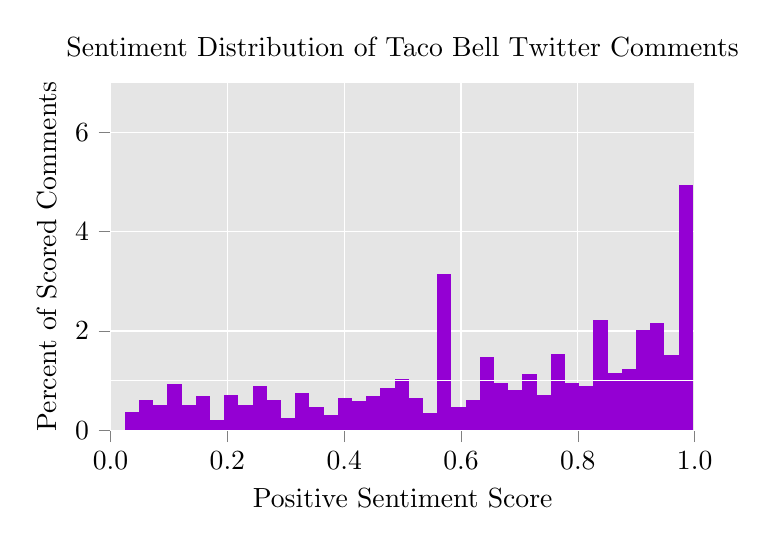
\begin{tikzpicture}

\definecolor{color0}{rgb}{0.580392156862745,0,0.827450980392157}

\begin{axis}[
axis background/.style={fill=white!89.80392156862746!black},
axis line style={white},
height=6cm,
tick align=outside,
tick pos=left,
title={Sentiment Distribution of Taco Bell Twitter Comments},
width=9cm,
x grid style={white},
xlabel={Positive Sentiment Score},
xmajorgrids,
xmin=0, xmax=1,
xtick={0,0.2,0.4,0.6,0.8,1},
xticklabels={0.0,0.2,0.4,0.6,0.8,1.0},
y grid style={white},
ylabel={Percent of Scored Comments},
ymajorgrids,
ymin=0, ymax=7
]
\draw[fill=color0,draw opacity=0] (axis cs:0.0242587197571993,0) rectangle (axis cs:0.048572301864624,0.376704460881885);
\draw[fill=color0,draw opacity=0] (axis cs:0.048572301864624,0) rectangle (axis cs:0.0728858858346939,0.616425386995312);
\draw[fill=color0,draw opacity=0] (axis cs:0.0728858858346939,0) rectangle (axis cs:0.0971994623541832,0.513687979909073);
\draw[fill=color0,draw opacity=0] (axis cs:0.0971994623541832,0) rectangle (axis cs:0.121513046324253,0.924638080492968);
\draw[fill=color0,draw opacity=0] (axis cs:0.121513053774834,0) rectangle (axis cs:0.145826637744904,0.513687979909073);
\draw[fill=color0,draw opacity=0] (axis cs:0.145826637744904,0) rectangle (axis cs:0.170140221714973,0.684917096661458);
\draw[fill=color0,draw opacity=0] (axis cs:0.170140206813812,0) rectangle (axis cs:0.194453790783882,0.205475128998437);
\draw[fill=color0,draw opacity=0] (axis cs:0.194453805685043,0) rectangle (axis cs:0.218767389655113,0.71916295149453);
\draw[fill=color0,draw opacity=0] (axis cs:0.218767374753952,0) rectangle (axis cs:0.243080958724022,0.513687822496093);
\draw[fill=color0,draw opacity=0] (axis cs:0.243080973625183,0) rectangle (axis cs:0.267394542694092,0.890392225659895);
\draw[fill=color0,draw opacity=0] (axis cs:0.267394542694092,0) rectangle (axis cs:0.291708111763,0.616425764786579);
\draw[fill=color0,draw opacity=0] (axis cs:0.291708111763,0) rectangle (axis cs:0.316021710634232,0.239720836912864);
\draw[fill=color0,draw opacity=0] (axis cs:0.316021710634232,0) rectangle (axis cs:0.34033527970314,0.753409268072485);
\draw[fill=color0,draw opacity=0] (axis cs:0.34033527970314,0) rectangle (axis cs:0.364648848772049,0.479442261500672);
\draw[fill=color0,draw opacity=0] (axis cs:0.364648878574371,0) rectangle (axis cs:0.388962477445602,0.308212504602254);
\draw[fill=color0,draw opacity=0] (axis cs:0.38896244764328,0) rectangle (axis cs:0.413276016712189,0.650671640608055);
\draw[fill=color0,draw opacity=0] (axis cs:0.413276016712189,0) rectangle (axis cs:0.43758961558342,0.582179175359813);
\draw[fill=color0,draw opacity=0] (axis cs:0.43758961558342,0) rectangle (axis cs:0.461903184652328,0.684917516429532);
\draw[fill=color0,draw opacity=0] (axis cs:0.461903184652328,0) rectangle (axis cs:0.486216753721237,0.856146895536915);
\draw[fill=color0,draw opacity=0] (axis cs:0.48621678352356,0) rectangle (axis cs:0.510530352592468,1.02737501534085);
\draw[fill=color0,draw opacity=0] (axis cs:0.510530352592468,0) rectangle (axis cs:0.534843921661377,0.650671640608055);
\draw[fill=color0,draw opacity=0] (axis cs:0.534843921661377,0) rectangle (axis cs:0.559157490730286,0.342458758214766);
\draw[fill=color0,draw opacity=0] (axis cs:0.559157490730286,0) rectangle (axis cs:0.583471119403839,3.15061285185748);
\draw[fill=color0,draw opacity=0] (axis cs:0.583471119403839,0) rectangle (axis cs:0.607784688472748,0.479442261500672);
\draw[fill=color0,draw opacity=0] (axis cs:0.607784688472748,0) rectangle (axis cs:0.632098257541656,0.616425764786579);
\draw[fill=color0,draw opacity=0] (axis cs:0.632098257541656,0) rectangle (axis cs:0.656411826610565,1.47257266032349);
\draw[fill=color0,draw opacity=0] (axis cs:0.656411826610565,0) rectangle (axis cs:0.680725395679474,0.958884523001344);
\draw[fill=color0,draw opacity=0] (axis cs:0.680725336074829,0) rectangle (axis cs:0.705038964748383,0.821899004832387);
\draw[fill=color0,draw opacity=0] (axis cs:0.705039024353027,0) rectangle (axis cs:0.729352593421936,1.13011390210873);
\draw[fill=color0,draw opacity=0] (axis cs:0.729352593421936,0) rectangle (axis cs:0.753666162490845,0.719163392251008);
\draw[fill=color0,draw opacity=0] (axis cs:0.753666162490845,0) rectangle (axis cs:0.777979731559753,1.54106441196645);
\draw[fill=color0,draw opacity=0] (axis cs:0.777979731559753,0) rectangle (axis cs:0.802293300628662,0.958884523001344);
\draw[fill=color0,draw opacity=0] (axis cs:0.802293300628662,0) rectangle (axis cs:0.826606929302216,0.890390588568419);
\draw[fill=color0,draw opacity=0] (axis cs:0.826606929302216,0) rectangle (axis cs:0.850920498371124,2.22598192839598);
\draw[fill=color0,draw opacity=0] (axis cs:0.850920498371124,0) rectangle (axis cs:0.875234067440033,1.1643597779302);
\draw[fill=color0,draw opacity=0] (axis cs:0.875234067440033,0) rectangle (axis cs:0.899547636508942,1.23285152957316);
\draw[fill=color0,draw opacity=0] (axis cs:0.899547636508942,0) rectangle (axis cs:0.92386120557785,2.02050667346712);
\draw[fill=color0,draw opacity=0] (axis cs:0.923861145973206,0) rectangle (axis cs:0.948174774646759,2.15748488768502);
\draw[fill=color0,draw opacity=0] (axis cs:0.948174834251404,0) rectangle (axis cs:0.972488403320312,1.50681853614497);
\draw[fill=color0,draw opacity=0] (axis cs:0.972488403320312,0) rectangle (axis cs:0.996801972389221,4.93140611829263);
\path [draw=white, fill opacity=0] (axis cs:0,0)
--(axis cs:0,7);

\path [draw=white, fill opacity=0] (axis cs:1,0)
--(axis cs:1,7);

\path [draw=white, fill opacity=0] (axis cs:0,0)
--(axis cs:1,0);

\path [draw=white, fill opacity=0] (axis cs:0,1)
--(axis cs:1,1);

\end{axis}
\label{tacot}
\end{tikzpicture}